\section{Platform and Acquisition Workflow}
\label{sec:platform}

\begin{figure*}[t]
    \centering
    % \begin{subfigure}[b]{0.48\textwidth}
    %     \centering
    %     \includegraphics[width=\linewidth]{figures/techtile-room-overview.jpg}
    %     \caption{Wide view of the Techtile measurement room used for the campaign.}
    % \end{subfigure}
    % \hfill
    \begin{subfigure}[t]{0.48\textwidth}
        \centering
        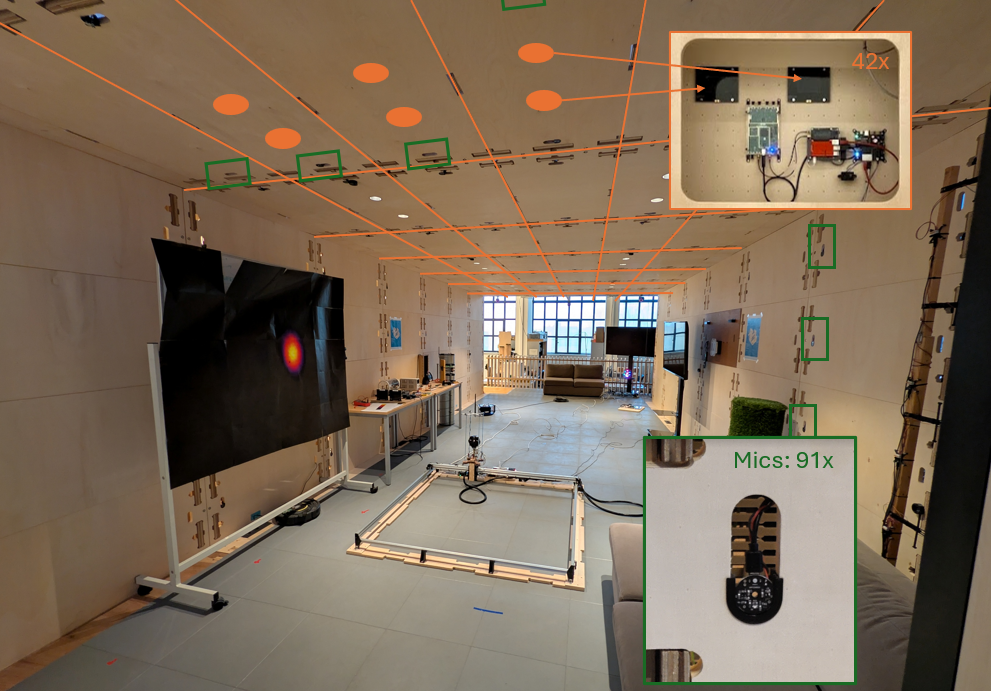
\includegraphics[height=5cm]{figures/techtile-room-setup.png}
        \caption{Measurement setup showing the rover frame and room instrumentation.}
    \end{subfigure}\hspace{2cm}%
    \begin{subfigure}[t]{0.32\textwidth}
        \centering
        \includegraphics[height=5cm]{figures/holder.jpg}
        \caption{Close-up of the rover-mounted payload combining the \gls{rf} antenna and the omnidirectional acoustic speaker on a common holder.}\label{fig:rover}
    \end{subfigure}
    \caption{Visual overview of the ARFT measurement setup, from room-scale deployment to the co-located RF-acoustic payload on the rover. \vspace{-3mm}}
    \label{fig:measurement-setup-photos}
\end{figure*}

ARFT is collected inside Techtile, a room-scale distributed testbed intended for communication, sensing, positioning, and related 6G experiments~\cite{techtilePrimer,techtileOpen6g, techtile-acoustic}. Techtile is built around 140 detachable tiles with Ethernet-based power, communication, and synchronization. It featurs a Qualisys-based sub-centimeter tracking system, 2D sampling robot, and 42 phase-coherent antennas operating at 920~MHz~\cite{syncWptTechtile,geomWpt2026,dliSuppression2026}. The transmit antenna is not phase-coherent with the receiving antennas.\footnote{This implies that the phase information should be interpreted relative to the other recived phases and should not be considered absolute. For instance, to determine the path length using the phase rotation between the transmitter and receiver.} For the campaign documented in this paper, the measurement rig (\cref{fig:rover}) combines an ultrasonic speaker and an \gls{rf} \gls{ue} antenna on a common mechanical mount so that the acoustic and \gls{rf} channels are sampled at the same physical 2D rover location. Ground-truth position is provided by the Qualisys system. The physical measurement environment is illustrated in \cref{fig:measurement-setup-photos}.



\subsection{Positioning and Measurement Procedure}

The measurements are coordinated by a central orchestrator, that coordinates the movement of the rover, position acquisition and RF and acoustic sampling.

\subsubsection{Orchestator}
The acquisition stack is organized around two control layers. The deployment layer pushes code and settings to the clients and starts the long-lived services. The orchestration layer then coordinates one end-to-end measurement cycle across rover motion, position logging, acoustics, and \gls{rf} synchronization. 
First, the rover moves to the commanded waypoint. Then the system records one fresh ground-truth Qualisys position sample at that stop. Afterward, the acoustic client records one chirp-response capture. Finally, the \gls{rf} orchestrator triggers one synchronized \gls{rf} cycle across the participating radio elements.

\subsubsection{Rover}
Both an antenna and speaker are mounted on a rover xy-plotter, as depicted in \cref{fig:rover}. The rover follows a reproducible multi-resolution scan over an $1.23 \times 1.23$~m work area. It performs a sweep over the area and with each iterations the density increases. Hence, the density of the collected samples is related to the total measurement time per area. This can be observed in \cref{fig:samples}. In particular, the rover planner uses a square spiral seven-sweep multi-resolution scan whose spacing is progressively reduced from 120 mm to approximately 50 mm. This makes the measurement process dense enough for spatial visualization while remaining operationally tractable for a multi-modal campaign.

\begin{figure}[t]
    \centering
    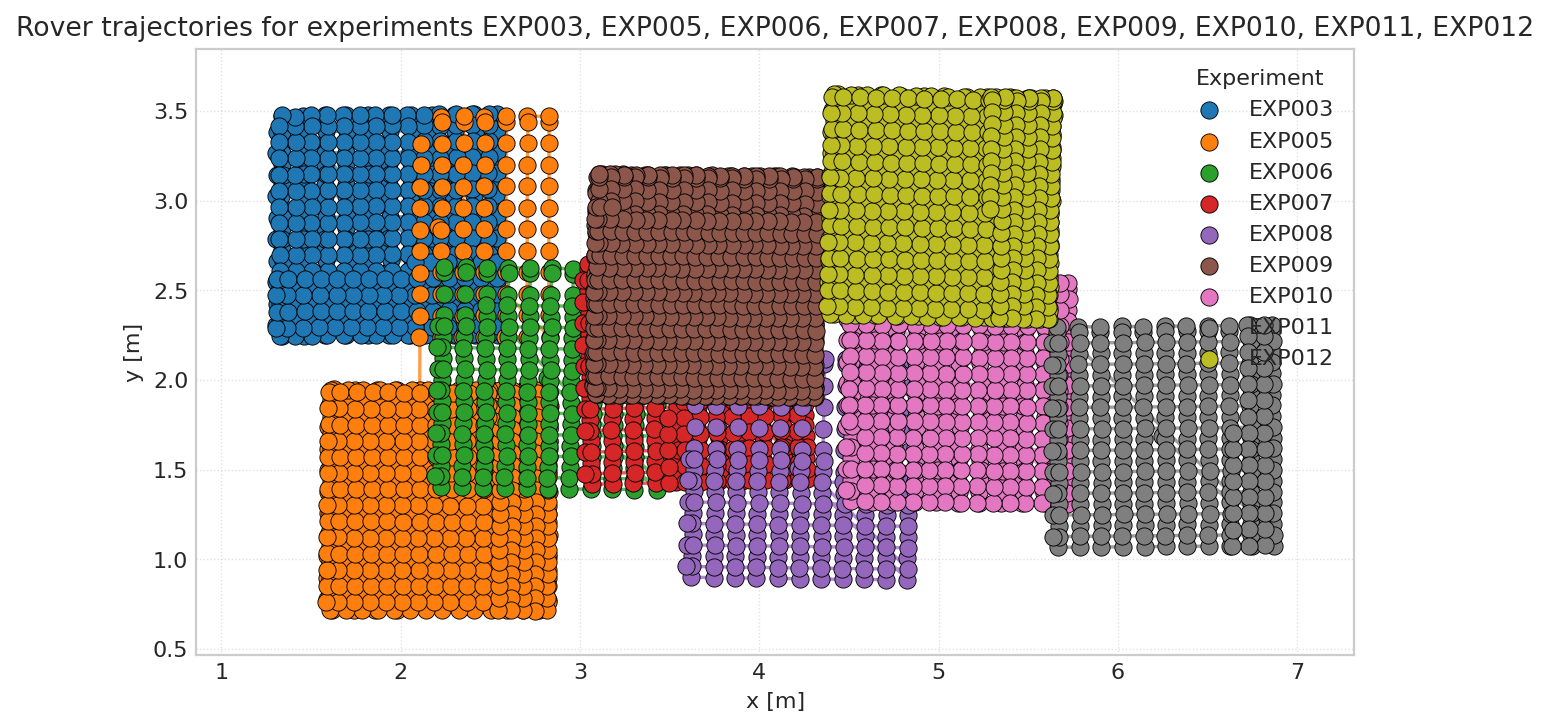
\includegraphics[width=\linewidth]{figures/notebook-exports/measurement_locations_trajectory.png}
    \caption{Trajectory and sampled measurement locations. \vspace{-3mm}}\label{fig:samples}
\end{figure}

\subsubsection{Positioning Ground Truth}
Ground-truth positioning is provided by the Qualisys system. 6 Miqus M3 cameras are installed, resulting in a 3D standard deviation on the accuracy of 1.25 mm.  After every completed rover move, the orchestrator requests one fresh $(x,y,z)$ position update. Note that in this dataset, the rover only moves in the $(x,y)$ plane, but the $z$-coordinates are stored as well. The reported $z$-coordinate is positioned at the bottom of the transmitter antenna.

\subsection{RF Orchestrator and Measurements}

The active \gls{rf} aperture used by the reciprocity workflow is the Techtile ceiling group: 42 receiver tiles\footnote{
Column \texttt{A} until \texttt{G} and row 5 until 10, covering \texttt{A05} until \texttt{G10}}. The campaign configuration uses the \gls{rf} measurements at 920~MHz with a 250~kS/s sample rate and receiver gain of 80.  

At each rover stop, the \gls{rf} orchestrator waits for an \texttt{ALIVE}  from all the tiles, publishes a  \texttt{SYNC} message, and waits for the corresponding \texttt{DONE} quorum before reporting completion to the main orchestrator. Techtile is further synchronized via a pulse-per-second distribution for time alignment, a shared 10~MHz reference for frequency alignment, and reciprocity-based calibration for front-end phase alignment~\cite{syncWptTechtile}. 

Each receiver stores one pilot-response record per cycle containing the measured pilot phase and amplitude. The reciprocity client estimates a circular-mean pilot phase from the captured IQ samples and pairs it with an \gls{rms} pilot amplitude, post-processing then applies cable-phase correction and converts the result into one complex \gls{csi} value per ceiling antenna. A single physical stop therefore produces a vector of up to 42 phase-coherent complex \gls{csi} observations across the active ceiling receivers. Currently, the dataset is limited to single-band \gls{csi} only.

\subsection{Acoustic Measurements}
The acoustic modality uses the rover-mounted ultrasonic speaker as the active source and the 91 distributed room microphones as fixed receivers. An opposite acoustic dataset in the same environment with the speakers being the anchors and a microphone being the mobile node was used and presented in~\cite{Echoes_of_accuracy, dataset_ultrasound_techtile}. Here, the speaker combines multiple Kemo L010 speakers in a dodecahedron shape forming a quasi-omni-directional ultrasonic speaker. The custom build microphone modules consist of IMP23ABSU \gls{mems} microphones combined with a pure analogue amplifier. One acoustic capture emits a 30~ms linear chirp from 20 to 40~kHz at a 250~kS/s sample rate. The acquisition task records a window twice as long as the excitation so that the direct arrival and the multipath components are preserved in the received signal to make the dataset more usable. The acoustic parameters of the Techtile environment were reported in~\cite{techtile-acoustic}. Techtile is a challenging environment in acoustic terms, with high reverberation and external noise factors. Due to the reverberation time ($\text{RT}_{60}$) of 0.4 s, an acoustic measurement can only take place with this low update rate to exclude interference across measurements. Therefore the acoustic data should be handled as a static dataset. In the current release configuration, these received chirp signals are stored directly rather than being reduced to only deconvolved impulse responses.

On the hardware side, the acoustic hardware shares the same \gls{daq} and thus reference clock, ensuring nanosecond synchronization between output and input tasks. A hardware start triggering ensures that the speaker emission and microphone sampling are aligned within one capture. Each saved acoustic data capture stores the chirp settings together with a microphone label, microphone coordinates, and the recorded waveform samples. The acoustic parser later reorganizes these runtime files into per-experiment waveform tensors indexed by experiment, cycle, microphone label, and sample index. Because the acoustic source and the \gls{rf} antenna are co-located on the rover, the acoustic traces and \gls{rf} snapshots refer to the same physical rover pose, except for a $z$-dimension offset as depicted in Fig.~\ref{fig:measurement-setup-photos} 

\begin{table}[t]
    \centering
    \caption{Key acquisition settings reconstructed from the campaign configuration.}
    \label{tab:config}
    \setlength{\tabcolsep}{4pt}
    \begin{tabular}{p{0.42\columnwidth}p{0.5\columnwidth}}
        \toprule
        Parameter & Value \\
        \midrule
        Testbed & Techtile distributed room-scale infrastructure \\
        Active \gls{rf} aperture & 42 ceiling receiver tiles (\texttt{A05}--\texttt{G10}) \\
        \gls{rf} excitation & Continious waveform pilot \\
        Center frequency & 920 MHz \\
        RF sample rate & 250 kS/s \\
        Receiver gain & 80 \\
        Positioning system & Qualisys \\
        Acoustic rig & ultrasonic speaker co-mounted with the \gls{rf} antenna, 91 microphones in walls and ceiling \\
        Acoustic excitation & 20--40 kHz linear chirp, 30 ms at 250 kS/s \\
        Runtime recording & rover CSV logs with pose, per-host \gls{rf} pilot logs, per-cycle acoustic waveform captures \\
        Rover sweep plan & 7 sweeps with nominal spacings 120, 120, 90, 90, 67.5, 67.5, and 50.6 mm\\
        \gls{rf} sync group & 43 synchronized subscribers in the pilot-synchronization loop \\
        Cycle semantics & 1 rover stop + 1 position sample + 1 acoustic capture + 1 \gls{rf} cycle \\
        \bottomrule
    \end{tabular}
\end{table}

\Cref{tab:config} highlights the key acquisition setting that were used to collect the ARFT dataset. Post-processing begins after acquisition. The \gls{rf} parser scans the per-host result files, extracts complex pilot measurements, applies cable correction, joins the result with rover positions, filters consecutive duplicate positions using a tolerance derived from the rover configuration, and writes one merged NetCDF. The acoustic parser produces a separate per-experiment NetCDF of recorded waveforms. ARFT therefore preserves both the runtime logs and the processed analysis data. The latter ultimately forms the merged dataset.
